\documentclass{beamer}
\mode<presentation> {
  % The Beamer class comes with a number of default slide themes
  % which change the colors and layouts of slides. Below this is a list
  % of all the themes, uncomment each in turn to see what they look like.
  
  %\usetheme{default}
  %\usetheme{AnnArbor}
  %\usetheme{Antibes}
  %\usetheme{Bergen}
  %\usetheme{Berkeley}
  %\usetheme{Berlin}
  %\usetheme{Boadilla}
  %\usetheme{CambridgeUS}
  %\usetheme{Copenhagen}
  %\usetheme{Darmstadt}
  %\usetheme{Dresden}
  \usetheme{Frankfurt}
  %\usetheme{Goettingen}
  %\usetheme{Hannover}
  %\usetheme{Ilmenau}
  %\usetheme{JuanLesPins}
  %\usetheme{Luebeck}
  %\usetheme{Madrid}
  %\usetheme{Malmoe}
  %\usetheme{Marburg}
  %\usetheme{Montpellier}
  %\usetheme{PaloAlto}
  %\usetheme{Pittsburgh}
  %\usetheme{Rochester}
  %\usetheme{Singapore}
  %\usetheme{Szeged}
  %\usetheme{Warsaw}
  % As well as themes, the Beamer class has a number of color themes
  % for any slide theme. Uncomment each of these in turn to see how it
  % changes the colors of your current slide theme.
  
  %\usecolortheme{albatross}
  %\usecolortheme{beaver}
  %\usecolortheme{beetle}
  %\usecolortheme{crane}
  %\usecolortheme{dolphin}
  %\usecolortheme{dove}
  %\usecolortheme{fly}
  %\usecolortheme{lily}
  %\usecolortheme{orchid}
  %\usecolortheme{rose}
  %\usecolortheme{seagull}
  %\usecolortheme{seahorse}
  %\usecolortheme{whale}
  %\usecolortheme{wolverine}
  
  %\setbeamertemplate{footline} % To remove the footer line in all slides uncomment this line
  %\setbeamertemplate{footline}[page number] % To replace the footer line in all slides with a simple slide count uncomment this line
  
  %\setbeamertemplate{navigation symbols}{} % To remove the navigation symbols from the bottom of all slides uncomment this line
}
\newcommand{\R}{\mathbb{R}}

\newcommand{\N}{\mathbb{N}}
\newcommand{\E}{\mathrm{E}}
\newcommand{\dif}{\textrm{d}}
\usepackage{url,bm}
\usepackage{cancel} 
\usepackage{amsmath}
\usepackage{mathrsfs}
\usepackage{mathbbol}
\usepackage{wrapfig}
\usepackage{graphicx} % Allows including images
\usepackage{booktabs} % Allows the use of \toprule, \midrule and \bottomrule in tables
\usepackage{listings}
\usepackage{color} %red, green, blue, yellow, cyan, magenta, black, white
\definecolor{mygreen}{RGB}{28,172,0} % color values Red, Green, Blue
\definecolor{mylilas}{RGB}{170,55,241}
\lstset{language=Matlab,%
%basicstyle=\color{red},
breaklines=true,%
morekeywords={matlab2tikz},
keywordstyle=\color{blue},%
morekeywords=[2]{1}, keywordstyle=[2]{\color{black}},
identifierstyle=\color{black},%
stringstyle=\color{mylilas},
commentstyle=\color{mygreen},%
showstringspaces=true,%without this there will be a symbol in the places where there is a space
numbers=left,%
numberstyle={\tiny \color{black}},% size of the numbers
numbersep=9pt, % this defines how far the numbers are from the text
emph=[1]{for,end,break},emphstyle=[1]\color{red}, %some words to emphasise
%emph=[2]{word1,word2}, emphstyle=[2]{style},    
}
%----------------------------------------------------------------------------------------
  %	TITLE PAGE
%----------------------------------------------------------------------------------------
  
  \title[Short title]{Factor analysis} % The short title appears at the bottom of every slide, the full title is only on the title page

\author{}
% Your name
\institute[NCU] % Your institution as it will appear on the bottom of every slide, may be shorthand to save space
{
  National Central University % Your email address
}
\date{\today} % Date, can be changed to a custom date

\begin{document}

\begin{frame}
\titlepage % Print the title page as the first slide
\end{frame}

\begin{frame}
\frametitle{Outline} 
\tableofcontents
\end{frame}

%----------------------------------------------------------------------------------------
  %	PRESENTATION SLIDES
%----------------------------------------------------------------------------------------
  
  %------------------------------------------------
\section{Introduction} % Sections can be created in order to organize your presentation into discrete blocks, all sections and subsections are automatically printed in the table of contents as an overview of the talk
%------------------------------------------------
\subsection{Motivation} 
\begin{frame}
\frametitle{Motivation example (Using a Regression example)}
For children in elementrays school\\
\textbf{Observed variable}:Shoe size and reading ability
\begin{wrapfigure}{r}{0.5\textwidth}
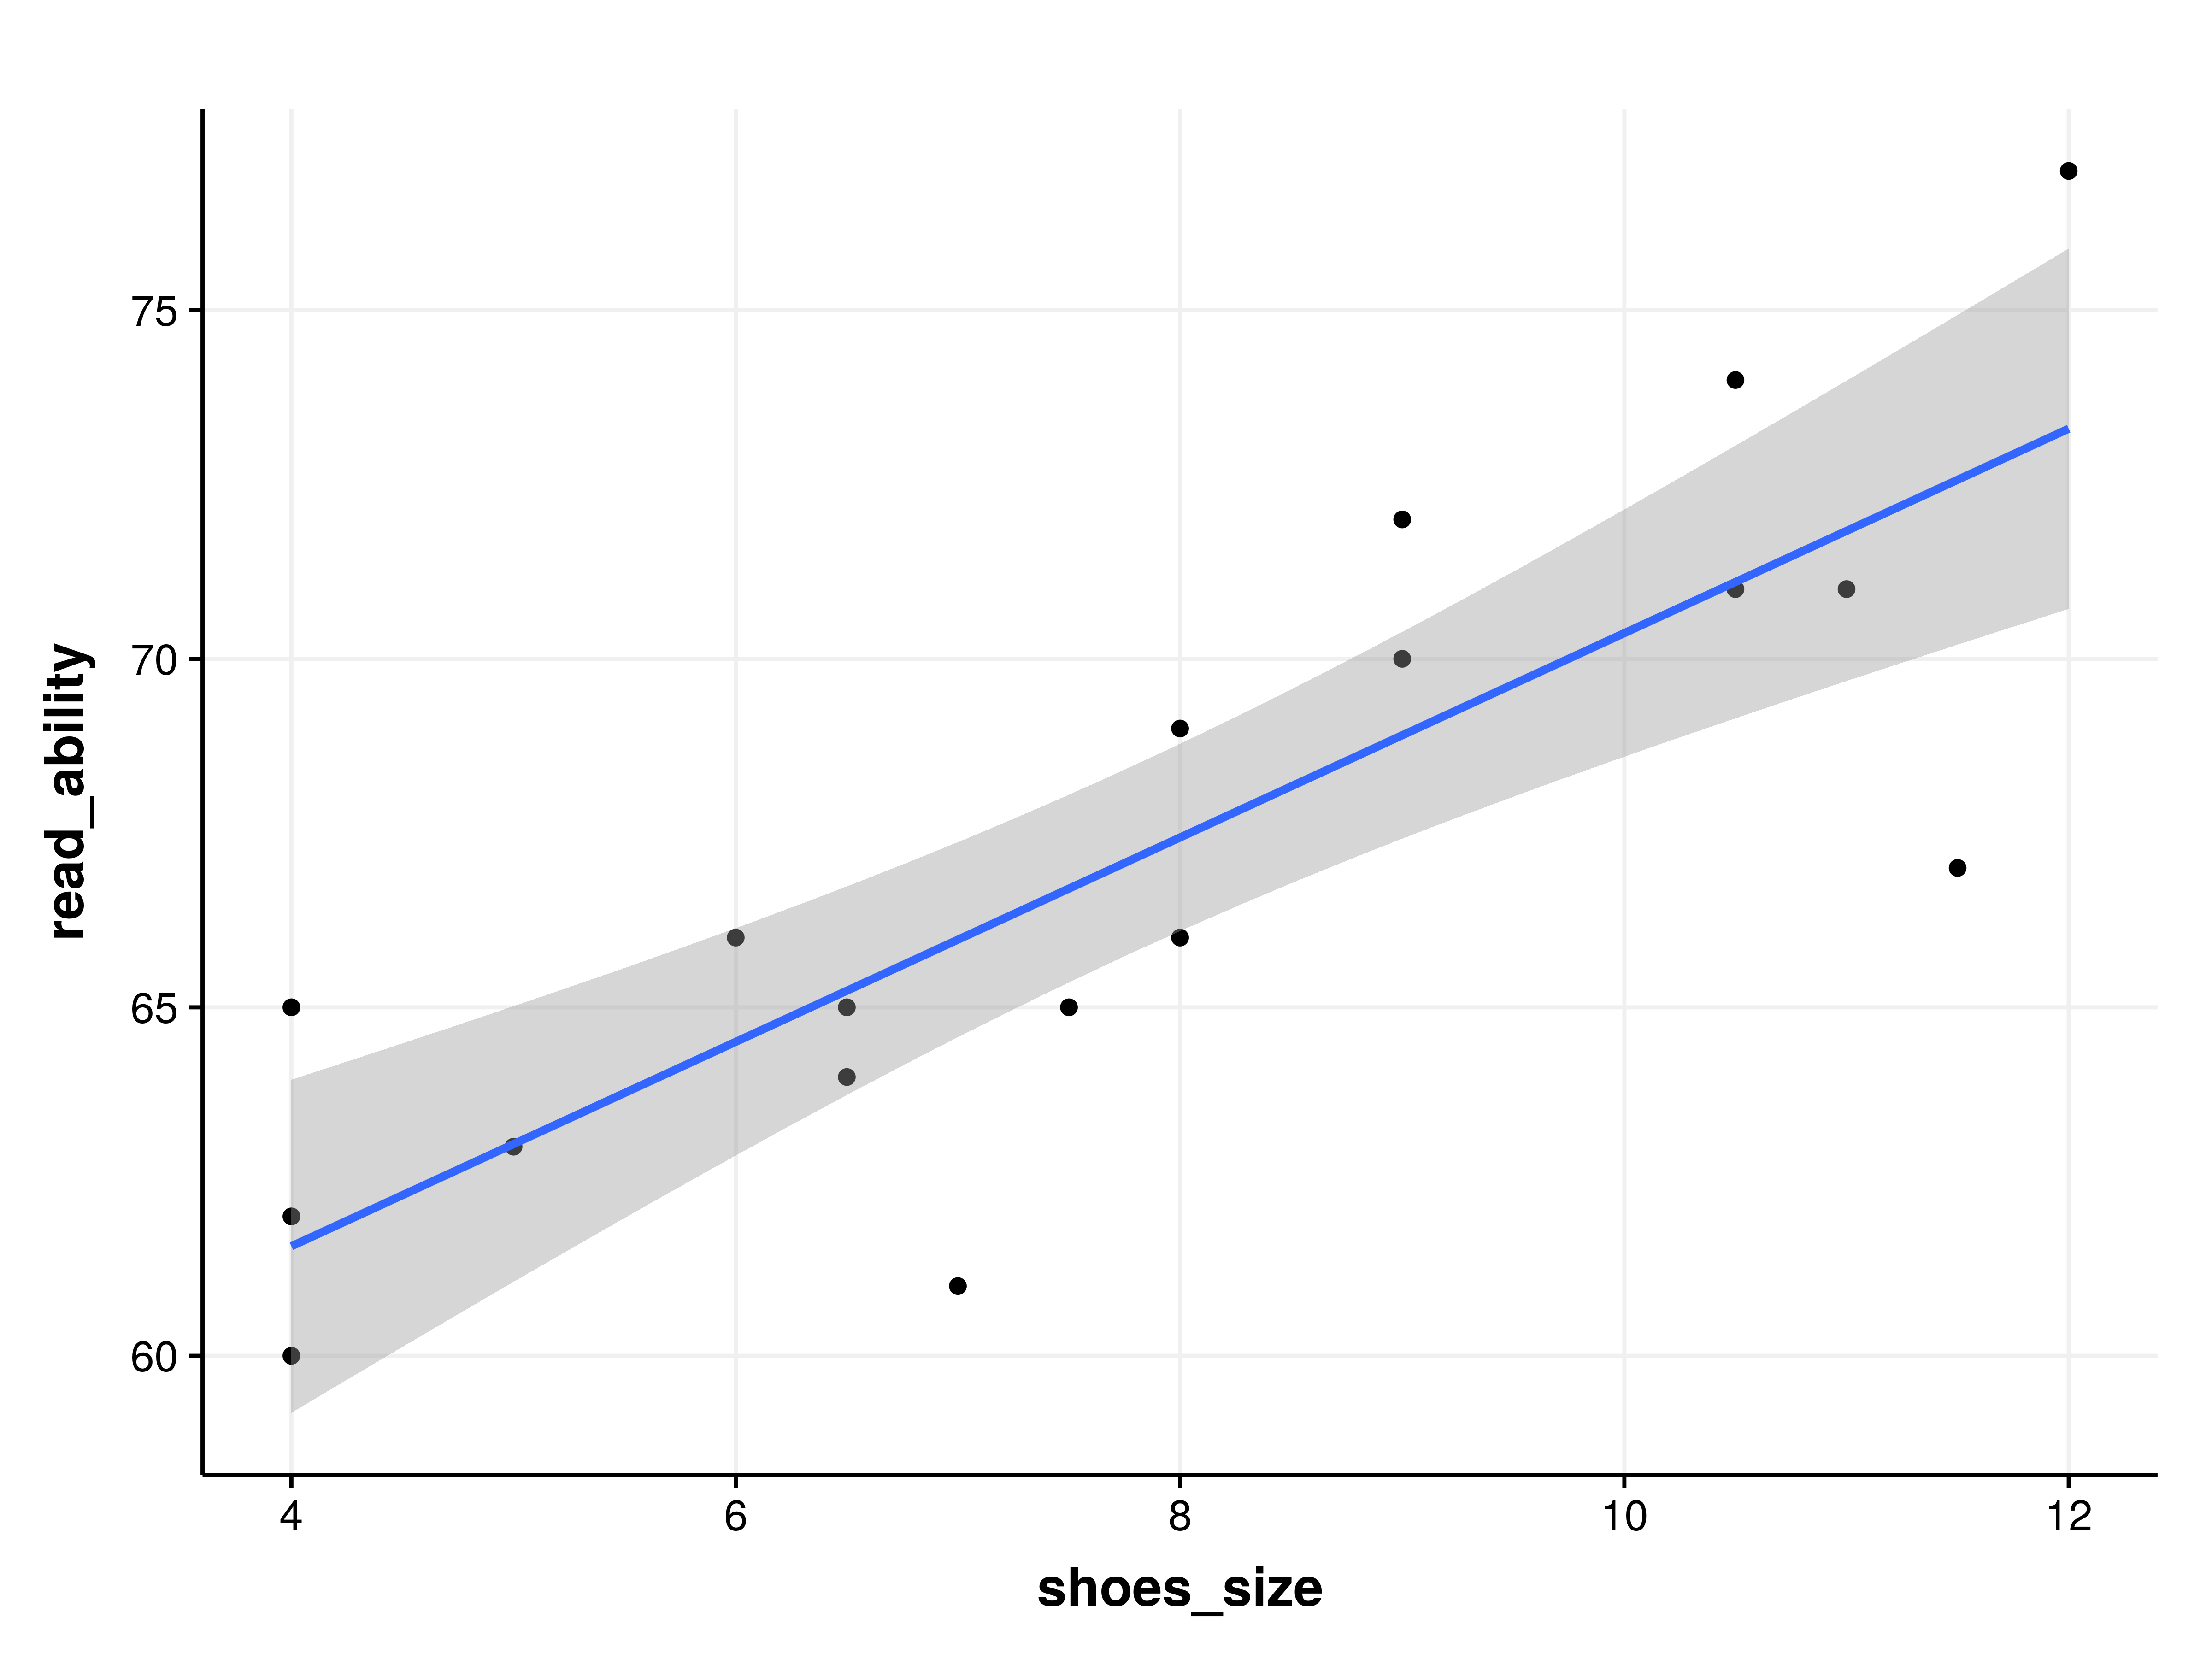
\includegraphics[width=4cm]{shoe.png}
\centering
\end{wrapfigure}
\textbf{latent variable}: age
\end{frame}
\subsection{Purpose of factor analysis} 
\begin{frame}
\frametitle{Purpose of factor analysis}
\begin{itemize}
\item Dimension reduction (it is not the most important in factor analysis)
\item Describe the  covariance relationship among many observable vaiables in terms of a few underlying, but unobservable (latent) variable.
\end{itemize}
\end{frame}
\frametitle{Group}

\section{Modeling}
\subsection{The Orthogonal Factor Model}
\begin{frame}
\frametitle{The Orthogonal Factor Model}
The observable random vector $\bm{X}$, with components has mean $\bf{\mu}$ and covariance matrix 
  $\Sigma$. $\bm{X}$ is linearly dependent upon a few unobservable random variables 
$F_1,F_2,\ldots, F_m$ called \textcolor{red}{common factor}
{\footnotesize
\begin{align*}
X_1-\mu_1&=\ell_{11}F_1+\ell_{12}F_2+\cdots+\ell_{1m}F_m+\varepsilon_1\\
X_2-\mu_2&=\ell_{21}F_1+\ell_{22}F_2+\cdots+\ell_{2m}F_m+\varepsilon_2\\
		 &\vdots\\
X_p-\mu_p&=\ell_{p1}F_1+\ell_{p2}F_2+\cdots+\ell_{pm}F_m+\varepsilon_p
\intertext{in matrix notation}
\bm{X}-\bm{\mu}&=\bm{LF}+\bm{\varepsilon}
\end{align*}
}
Assume that
\begin{align*}
&\E(\bm{F})=\bm{0}_{(m\times 1)},\mbox{Cov}(\bm{F})=\E(\bm{FF^{\prime}})=\mathbb{I}_{(m\times m)}
\\
&\E(\bm{\varepsilon})=\bm{0}_{(p\times 1)},
\mbox{Cov}(\bm{\varepsilon})=\E(\bm{\bm{\varepsilon}\bm{\varepsilon}^{\prime}})=\varPsi_{(p\times p)}
\end{align*}
where $\varPsi$ is a diagonal matrix.
\end{frame}
\begin{frame}
So the covariance structure for $\bm{X}$ From this model 
  \begin{align*}
\Sigma
&=\mbox{Cov}(\bm{X})=\E\left((\bm{X}-\bm{\mu})(\bm{X}-\bm{\mu})^{\prime}\right)\\
&=\bm{L}\E(\bm{FF}^{\prime})\bm{L}^{\prime}+
\cancelto{0}{\E(\bm{\varepsilon F^{\prime}})\bm{L^{\prime}}}+
\cancelto{0}{\bm{L}\E(\bm{F\varepsilon}^{\prime})}+
\E(\bm{\varepsilon\varepsilon}^{\prime})\\
&=\bm{LL^{\prime}}+\varPsi
\end{align*}
\end{frame}
\section{Method}
\subsection{Principlal Component}
\begin{frame}
\end{frame}
\begin{frame}
\end{frame}
\subsection{MLE}
\begin{frame}
\end{frame}
\begin{frame}
\end{frame}
\section{Factor Analysis in R(Python)}
\begin{frame}
\end{frame}
\begin{frame}
\end{frame}
\section{Extended reading}
\begin{frame}
\end{frame}
\begin{frame}
\end{frame}

\end{document}